% Authors: Taejin Hwang, Justin Yu
% Emails: taejin@berkeley.edu, justinvyu@berkeley.edu

% Note: This specific reboot is specific to Sahai's Fall 2019 iteration of 16B. It was created by merging the bode_plots_intro and bode_filters question. For future semesters, it'll probably be more appropriate to use the two together.

\qns{Frequency Responses}
\pgfplotsset{compat=1.9, every tick label/.append style={font=\normalsize}} 

The transfer function of a circuit is defined as

\begin{equation}
H(j \omega) = \frac{\widetilde{V}_{out}}{\widetilde{V}_{in}}
\end{equation}

The transfer function depends on the frequency of the input voltage, and will be a complex number for a given frequency. 

When looking at filters, we will define a transfer function that explains the input-output relation for any given frequency and analyze its behavior. 
For the purposes of this question, we will consider various filter configurations, and study their behavior.

\begin{enumerate}

\qitem Given the following filter, with $R = 100 \Omega$ and $C = 100 pF,$

\begin{center}
  \begin{circuitikz} \draw
    (0, 0) node[ground] {}
      to [sV, l_=$V_{in}$] (0, 4)
      to [R = R] (4, 4)
      to [C = C] (4, 0)
      node[ground] {}

    (4, 3) to[short, -o] (6, 3) node[anchor=west] (A) {A}

    (4, 1) to[short, -o] (6, 1) node[anchor=west] (B) {B}

    (A) to[open, l^=$V_{out}$] (B)
  ;\end{circuitikz}
\end{center}


\begin{enumerate}[label=(\roman*)]
  \item \textbf{Write out the transfer function $H(j\omega)$.}
  \item \textbf{For values of $\omega$ approaching $0$, find $\abs{H(j\omega)}$.}
  \item \textbf{For values of $\omega$ approaching $\infty$, find $\abs{H(j\omega)}$.}
  \item \textbf{What is the cutoff frequency of this filter?}
  \item \textbf{Sketch its phase and magnitude.}
\end{enumerate}

\sol {

\begin{enumerate}[label=(\roman*)]
  \item The circuit can be simplified as:
    \input{\bank/filters/filter_transfer/fig_simplified_low_pass}

    We recognize the circuit is a voltage divider.
    Let $\widetilde{V}_{out}$ and $\widetilde{V}_{in}$ be voltage phasors.
    Using the voltage divider equation with impedance, we have
    \[
      \widetilde{V}_{out} = \frac{Z_C}{Z_R + Z_C}\widetilde{V}_{in} = H(j\omega)\widetilde{V}_{in}
    .\]
    Notice that the above equation uses impedance and voltage phasors instead of resistance and voltage.
    From the above equation, the circuit has the transfer function
    \[
      H(j\omega) = \frac{Z_C}{Z_R + Z_C}
      = \frac{\frac{1}{j\omega C}}{R + \frac{1}{j\omega C}}
      = \frac{1}{1 + j\omega RC}
    ,\]

  \item For values of $\omega$ close to $0$, $\abs{H(j\omega)}$ approaches $1$.
    In this case, $\widetilde{V}_{out} = \widetilde{V}_{in}$, meaning that low frequencies will pass through this filter.

  \item For values of $\omega$ approaching $\infty$, $\abs{H(j\omega)}$ approaches $0$.
    In this case, $\widetilde{V}_{out} = 0$, meaning that high frequencies will be attenuated by this filter.
    
    \vspace{0.1 cm} 

    Since this filter allows low frequencies to go through and blocks high frequencies, it is called a \emph{low-pass filter}.

  \item Recall that the cutoff frequency is the point at which the magnitude of $H(j \omega)$ is equal to $\frac{1}{\sqrt{2}}.$ 
  The reason for this values is since it is the "half-power" point. Since $H(j \omega) = \frac{1}{1 + j \omega RC},$ and noting that $\frac{1}{1 + j}$ has magnitude $\frac{1}{\sqrt{2}},$ we can solve for $\omega$ and get $\omega_{c} = \frac{1}{RC} = \frac{1}{10^{2} \cdot 10^{-10}} = 10^{8}$

  \item {
  Magnitude (log-log scale): The magnitude of $H(j \omega)$ is close to 1 until $\omega_{c}$, after which it starts decreasing at a quick rate.

  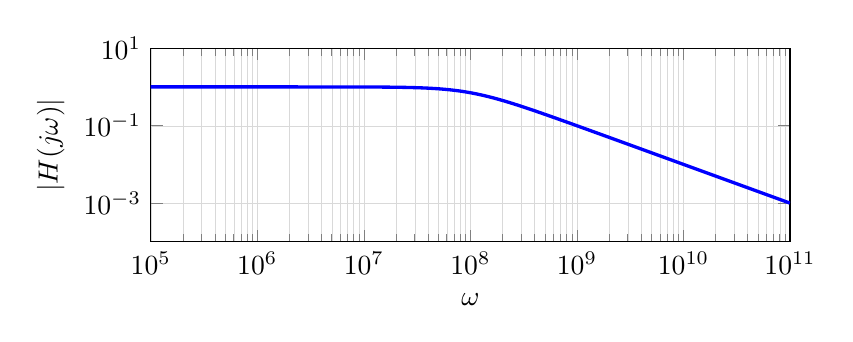
\begin{tikzpicture}[
    declare function={
      mag(\omega)= 1 / sqrt(1 + (\omega / 10^8)^2)
      % Bode approximation
      % (\omega < 10^8) * (1) +
      %           (\omega >= 10^8) * (10^8 / \omega)
     ;
    }
  ]
    \begin{loglogaxis}[
      ymin=0.0001, ymax=10, ylabel=$|H(j \omega)|$,
      xmin=10^5, xmax=10^11, xlabel=$\omega$,
      domain=10^5:10^11,
      grid=both, grid style={line width=.1pt, draw=gray!30},
      width=\textwidth * 0.8,
      height=\textwidth / 3,
      samples=800
    ]
      \addplot [blue,very thick] {mag(x)};
    \end{loglogaxis}
  \end{tikzpicture}
  
  Phase (semi-log scale): The phase of $H(j \omega)$ can be approximated using the three points from the previous parts. When $\omega << \omega_{c}, \angle H(j \omega) = 0,$ when $\omega = \omega_{c}, \angle H(j \omega) = \frac{\pi}{4},$ and when $\omega >> \omega_{c}, \angle H(j \omega) = \frac{\pi}{2}.$

  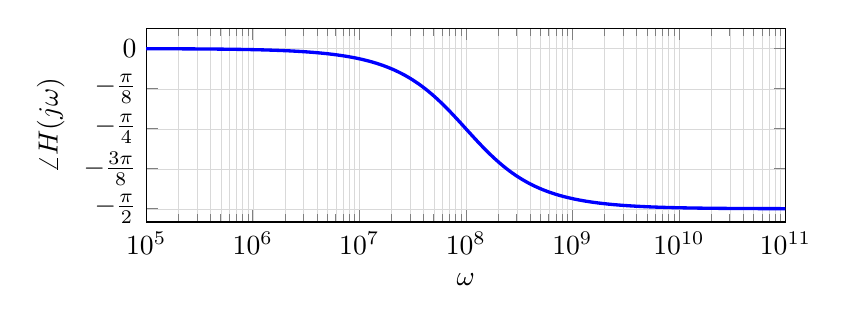
\begin{tikzpicture}[
    declare function={
      phase(\omega)= -rad(atan(\omega / 10^8))
      % Bode approximation
      % phase(\omega)= (\omega < 10^7) * (0) +
      %           and(\omega >= 10^7, \omega < 10^9) * (-pi / 4 * (log10(\omega) - 7)) +
      %           (\omega >= 10^9) * (-pi / 2)
      ;
    }
  ]
    \begin{semilogxaxis}[
      ymin= -1.7, ymax=0.2, ylabel=$\angle H(j \omega)$,
      ytick={-pi/2, -3*pi/8, -pi/4, -pi/8, 0},
      yticklabels={$-\frac{\pi}{2}$,$-\frac{3\pi}{8}$,$-\frac{\pi}{4}$,$-\frac{\pi}{8}$,$0$},
      xmin=10^5, xmax=10^11, xlabel=$\omega$,
      domain=10^5:10^11,
      grid=both, grid style={line width=.1pt, draw=gray!30},
      width=\textwidth * 0.8,
      height=\textwidth / 3,
      samples=800
    ]
      \addplot [blue,very thick] {phase(x)};
    \end{semilogxaxis}
  \end{tikzpicture}
  }
\end{enumerate}
}

\qitem Given the following filter, with $R = \SI{1}{\kilo\ohm}$ and $C = \SI{10}{\nano\farad},$

\begin{center}
  \begin{circuitikz} \draw
    (0, 0) node[ground] {}
      to [sV, l_=$v_{in}$] (0, 2)
      to [C = C] (4, 2)
      to [R = R] (4, 0)
      node[ground] {}

    (4, 2) to[short, -o] (5, 2) node[anchor=west] (A) {A}

    (4, 0) to[short, -o] (5, 0) node[anchor=west] (B) {B}

    (A) to[open, l^=$v_{out}$] (B)
  ;\end{circuitikz}
\end{center}


\begin{enumerate}[label=(\roman*)]
  \item \textbf{Write out the transfer function $H(j\omega)$.}
  \item \textbf{For values of $\omega$ approaching $0$, find $\abs{H(j\omega)}$.}
  \item \textbf{For values of $\omega$ approaching $\infty$, find $\abs{H(j\omega)}$.}
  \item \textbf{What is the cutoff frequency of this filter?}
  \item \textbf{Sketch its phase and magnitude.}
\end{enumerate}

\sol {
\begin{enumerate}[label=(\roman*)]
   \item The circuit can be simplified as:

    \begin{center}
  \begin{circuitikz}[american] \draw
    (0, 0) to[C, l=$C$] (2, 0) to[R, l=$R$] (2, -2) node[ground] {}
    (2, 0) to (3, 0) node[ocirc] {} node[right] {$V_{out}$}
    (0, 0) node[ocirc] {} node[left] {$V_{in}$}
  ;\end{circuitikz}
\end{center}


    Using the voltage divider equation with impedance, we have
    \[
      \widetilde{V}_{out} = \frac{Z_R}{Z_R + Z_C}\widetilde{V}_{in} = H(j \omega)\widetilde{V}_{in}
    .\]

    Thus, the circuit has the transfer function

    \[
      H(j \omega) = \frac{Z_R}{Z_R + Z_C}
      = \frac{R}{R + \frac{1}{j\omega C}}
      = \frac{j\omega RC}{1 + j\omega RC}
    .\]

  \item For values of $\omega$ close to $0$, $\abs{H(j \omega)}$ approaches $0$.
    In this case, $\widetilde{V}_{out} = 0$, it means that low frequencies will be attenuated by this filter.

  \item For values of $\omega$ approaching $\infty$, $\abs{H(j \omega)}$ approaches $1$.
    In this case, $\widetilde{V}_{out} = \widetilde{V}_{in}$, meaning high frequencies will pass through this filter.

    \vspace{0.1 cm} 

    Since this filter allows high frequencies to go through and blocks low frequencies, it is called a \emph{high-pass filter}.

  \item Doing a similar analysis as before, we can calculate $\omega_{c} = \frac{1}{RC} = \frac{1}{10^{3} \cdot 10^{-8}} = 10^{5}$

  \item 
  Magnitude (log-log scale): The magnitude of $H(j \omega)$ is close to 0 for $\omega$ close to 0. It will increase at a very slow rate

  until $\omega_{c}$, after which it starts increasing at a quick rate, but will asymptotically reach $1$ as $\omega >> \omega_{c}.$

  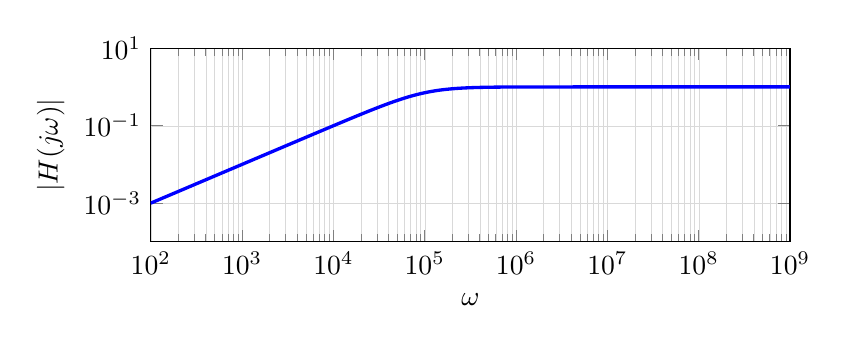
\begin{tikzpicture}[
    declare function={
    mag(\omega)= (\omega / 10^5) / sqrt(1 + (\omega / 10^5)^2)    
     %  Bode approximation
     %  mag(\omega)= (\omega < 10^5) * (\omega / 10^5) +
     %            (\omega >= 10^5) * (1)
     %
     ;
    }
  ]
    \begin{loglogaxis}[
      ymin=0.0001, ymax=10, ylabel=$|H(j \omega)|$,
      xmin=10^2, xmax=10^9, xlabel=$\omega$,
      domain=10^2:10^9,
      grid=both, grid style={line width=.1pt, draw=gray!30},
      width=\textwidth * 0.8,
      height=\textwidth / 3,
      samples=500
    ]
      \addplot [blue,very thick] {mag(x)};
    \end{loglogaxis}
    \vspace{0.3 cm}
  \end{tikzpicture}
  
  Phase (semi-log scale): The phase of $H(j \omega)$ is $\frac{\pi}{2}$ for $\omega << \omega_{c}.$ When $\omega = \omega_{c}, \angle H(j \omega) = \frac{\pi}{4},$ for larger values of $\omega,$ it will continue to decreases until it asymptotically reaches $0$ as $\omega >> \omega_{c}.$

  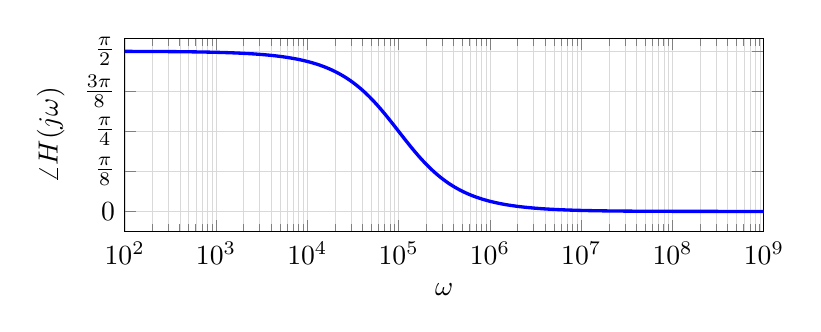
\begin{tikzpicture}[
    declare function={
    phase(\omega)= pi/2 - rad(atan(\omega / 10^5))
      % Bode approximation 
      % phase(\omega)= (\omega < 10^4) * (pi / 2) +
      %           and(\omega >= 10^4, \omega < 10^6) * (-pi / 4 * (log10(\omega) - 4) + pi / 2) +
      %           (\omega >= 10^6) * (0)
     ;
    }
  ]
  \begin{semilogxaxis}[
    ymin= -0.2, ymax=1.7, ylabel=$\angle H(j \omega)$,
    ytick={pi/2, 3*pi/8, pi/4, pi/8, 0},
    yticklabels={$\frac{\pi}{2}$,$\frac{3\pi}{8}$,$\frac{\pi}{4}$,$\frac{\pi}{8}$,$0$},
    xmin=10^2, xmax=10^9, xlabel=$\omega$,
    domain=10^2:10^9,
    grid=both, grid style={line width=.1pt, draw=gray!30},
    width=\textwidth * 0.8,
    height=\textwidth / 3,
    samples=500
  ]
    \addplot [blue,very thick] {phase(x)};
  \end{semilogxaxis}
\end{tikzpicture}

\end{enumerate}
}

\qitem Given the following filter, with $R_{1} = \SI{100}{\ohm}, R_{2} = \SI{1}{\kilo\ohm}$ and $C_{1} = \SI{100}{\pico\farad}, C_{2} = \SI{10}{\nano\farad},$

\begin{center}
  \begin{circuitikz} \draw
    (0, 2) node[ground] (lground) {}
      to [sV, l_=$v_{in}$] (0, 4)
      to [R = $R_1$] (4, 4)
      to [C = $C_1$] (4, 2)
      node[ground] (mground) {}

    (7, 3.5) node[op amp, yscale=-1] (opamp) {}
      (opamp.+) to [short] (4, 4)
      (opamp.-) -| (5.5, 2)
      (opamp.out) |- (5.5, 2)
      (opamp.out) to [C = $C_2$] (12, 3.5)
      to [R = $R_2$] (12, 0.5)
      node[ground] (rground) {}

    (12, 3.5) to[short, -o] (14, 3.5) node[anchor=west] (A) {A}

    (12, 1) to[short, -o] (14, 1) node[anchor=west] (B) {B}

    (A) to[open, l^=$v_{out}$] (B)
  ;\end{circuitikz}
\end{center}


\begin{enumerate}[label=(\roman*)]
  \item \textbf{Write out the transfer function $H(j\omega)$.}
  \item \textbf{For values of $\omega$ approaching $0$, find $\abs{H(j\omega)}$.}
  \item \textbf{For values of $\omega$ approaching $\infty$, find $\abs{H(j\omega)}$.}
  \item \textbf{What is the cutoff frequency of this filter?}
  \item \textbf{Sketch its phase and magnitude.}
\end{enumerate}

\sol {

\begin{enumerate}[label=(\roman*)]
\item The circuit can be simplified as:

    \begin{center}
  \begin{circuitikz}[american] \draw
    (5, -0.5) node[op amp, yscale=-1](opamp){}
    (0, 0) to[R, l=$R_1$] (2, 0) to[C, l=$C_1$] (2, -2) node[ground] {}
    (2, 0) to (3, 0) node[ocirc] {} node[above] {$V_{center}$} to (opamp.+)
    (0, 0) node[ocirc] {} node[left] {$V_{in}$}
    (6.5, 0) to[C, C=$C_2$] (8.5, 0) to[R, l=$R_2$] (8.5, -2) node[ground] {}
    (8.5, 0) to (9.5, 0) node[ocirc] {} node[right] {$V_{out}$}
    (0, 0) node[ocirc] {} node[left] {$V_{in}$}
    (opamp.-) to (3.5, -1) to (3.5, -2) to (6.5, -2) to (6.5, -0.5) to (opamp.out)
    (6.5, -0.5) to (6.5, 0)
  ;\end{circuitikz}
\end{center}


    In this circuit, the op-amp acts as a unity gain buffer which connects the two filters together.
    On the left of the op-amp is a low-pass filter, and on the right of the op-amp is a high-pass filter.
    Let $H_1(j \omega)$ and $H_2(j \omega)$ be transfer functions for the low-pass and high-pass filters respectively.
    We can write $\widetilde{V}_{out}$ in terms of $H_1(j \omega)$, $H_2(j \omega)$, and $\widetilde{V}_{in}$
    \[
      \widetilde{V}_{out} = H_1(j \omega)H_2(j \omega)\widetilde{V}_{in}
    .\]

    Thus, the circuit has the transfer function

    \[
      H(j \omega) = H_1(j \omega)H_2(j \omega) = \frac{1}{1 + j \omega R_{1}C_{1}} \frac{j \omega R_{2}C_{2}}{1 + j \omega R_{2}C_{2}}
    .\]


  \item Using the above transfer function, we have
    \[
      \abs{H(j \omega)} = \abs{H_1(j \omega)H_2(j \omega)}
      = \abs{H_1(j \omega)}\abs{H_2(j \omega)}
    .\]
    Since $H_1(j \omega)$ is a transfer function of a low-pass filter and $H_2(j \omega)$ is a transfer function of a high-pass filter, for values of $\omega$ approaching $0$, $\abs{H(j \omega)}$ approaches $0$.
    Therefore, $\widetilde{V}_{out} = 0$, meaning low frequencies are attenuated by this filter.

  \item For values of $\omega$ approaching $\infty$, $\abs{H(j \omega)}$ also approaches $0$.
    Therefore, $\widetilde{V}_{out} = 0$; meaning high frequencies are also attenuated by this filter. 

    \vspace{0.1 cm} 
    
    Since this filter blocks both low and high frequencies, and it allows signals of a certain frequency range (a band of frequencies) to pass through, it is called a \emph{band-pass filter}.
  \item What are the cutoff frequencies of this filter?

    The lower cutoff is the cutoff frequency of the high-pass filter:
    $$\omega_{c,h} = \frac{1}{R_{2}C_{2}} = 10^{5}$$
    The upper cutoff is the cutoff frequency of the low-pass filter:
    $$\omega_{c,l} = \frac{1}{R_{1}C_{1}} = 10^{8}$$
  \item Sketch its phase and magnitude. \textit{Hint: How can we combine the plots of the individual filters together?}

    For both the magnitude and the phase plots, you can "add" the plots of the high-pass filter and the low-pass filter.
    This can be done since both are on a log-log scale.
    \begin{figure}[h]
    \textbf{Magnitude plot:}
    \centering
      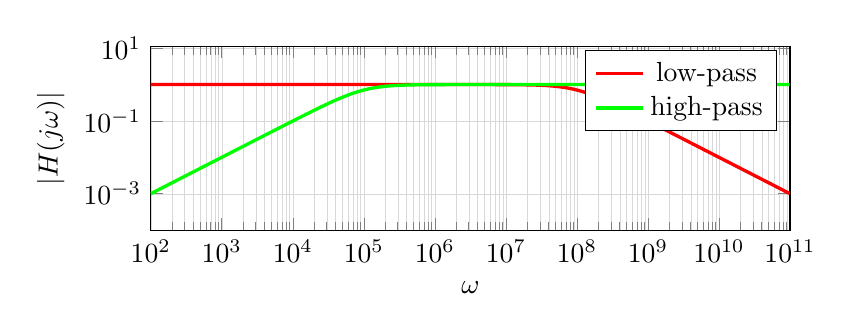
\begin{tikzpicture}[
        declare function={
         highpass(\omega)= (\omega / 10^5) * sqrt(1 + (\omega / 10^5)^2) / (1 + (\omega / 10^5)^2)
        % highpass(\omega)= (\omega < 10^5) * (\omega / 10^5) +
        %           (\omega >= 10^5) * (1)
        ;
        lowpass(\omega)= 1 / sqrt(1 + (\omega / 10^8)^2)
         % lowpass(\omega)= (\omega < 10^8) * (1) +
         %           (\omega >= 10^8) * (10^8 / \omega)
        ;
        }
      ]
        \begin{loglogaxis}[
          ymin=0.0001, ymax=11, ylabel=$|H(j \omega)|$,
          xmin=10^2, xmax=10^11, xlabel=$\omega$,
          domain=10^2:10^11,
          grid=both, grid style={line width=.1pt, draw=gray!30},
          width=\textwidth * 0.8,
          height=\textwidth / 3.1,
          samples=800
        ]
          \addplot [red,very thick] {lowpass(x)};
          \addlegendentry{low-pass}
          \addplot [green,very thick] {highpass(x)};
          \addlegendentry{high-pass}
        \end{loglogaxis}
      \end{tikzpicture}
    \end{figure}

    \begin{figure}
    \centering
      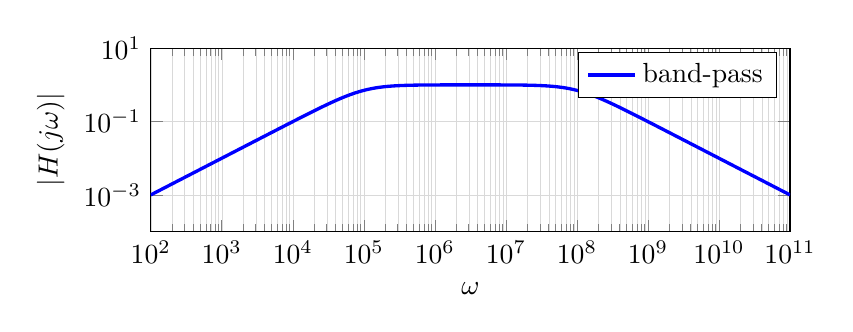
\begin{tikzpicture}[
        declare function={
        highpass(\omega)= (\omega / 10^5) / sqrt(1 + (\omega / 10^5)^2)
        % highpass(\omega)= (\omega < 10^5) * (\omega / 10^5) +
        %           (\omega >= 10^5) * (1)
        ;
        lowpass(\omega)= 1 / sqrt(1 + (\omega / 10^8)^2)
         % lowpass(\omega)= (\omega < 10^8) * (1) +
         %           (\omega >= 10^8) * (10^8 / \omega)
        ;
        }
      ]
        \begin{loglogaxis}[
          ymin=0.0001, ymax=10, ylabel=$|H(j \omega)|$,
          xmin=10^2, xmax=10^11, xlabel=$\omega$,
          domain=10^2:10^11,
          grid=both, grid style={line width=.1pt, draw=gray!30},
          width=\textwidth * 0.8,
          height=\textwidth / 3.1,
          samples=300
        ]
          \addplot [blue,very thick] {lowpass(x) * highpass(x)};
          \addlegendentry{band-pass}
          
        \end{loglogaxis}
      \end{tikzpicture}
    \end{figure}
    \newpage
    \begin{figure}[!h]
    \textbf{Phase plot:}
    \centering

      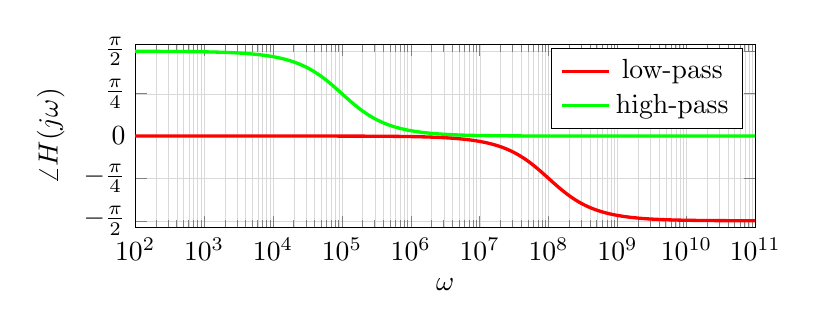
\begin{tikzpicture}[
        declare function={
        lowpass(\omega) = -rad(atan(\omega / 10^8))
          % lowpass(\omega)= (\omega < 10^7) * (0) +
          %           and(\omega >= 10^7, \omega < 10^9) * (-pi / 4 * (log10(\omega) - 7)) +
          %           (\omega >= 10^9) * (-pi / 2)
         ;
        highpass(\omega) = pi/2 - rad(atan(\omega / 10^5))
         % highpass(\omega)= (\omega < 10^4) * (pi / 2) +
         %           and(\omega >= 10^4, \omega < 10^6) * (-pi / 4 * (log10(\omega) - 4) + pi / 2) +
         %           (\omega >= 10^6) * (0)
        ;
        }
      ]

        \begin{semilogxaxis}[
          ymin= -1.7, ymax=1.7, ylabel=$\angle H(j \omega)$,
          ytick={-pi/2, -pi/4, 0, pi/4, pi/2},
          yticklabels={$-\frac{\pi}{2}$,$-\frac{\pi}{4}$,$0$,$\frac{\pi}{4}$,$\frac{\pi}{2}$},
          xmin=10^2, xmax=10^11, xlabel=$\omega$,
          domain=10^2:10^11,
          grid=both, grid style={line width=.1pt, draw=gray!30},
          width=\textwidth * 0.78,
          height=\textwidth / 3.1,
          samples=500
        ]
          \addplot [red,very thick] {lowpass(x)};
          \addlegendentry{low-pass}
          \addplot [green,very thick] {highpass(x)};
          \addlegendentry{high-pass}
        \end{semilogxaxis}
    \end{tikzpicture}
  \end{figure}

  \begin{figure}[!h]
  \centering

    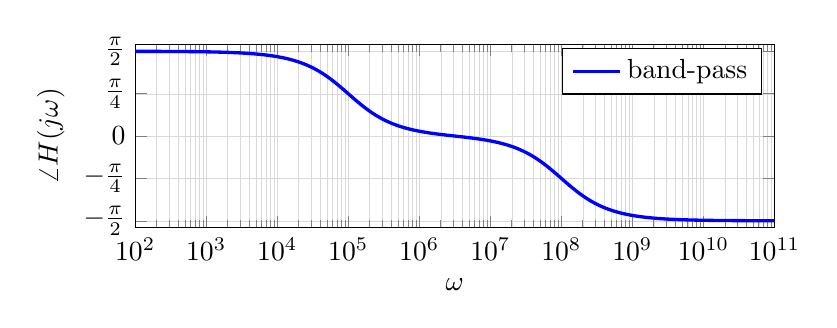
\begin{tikzpicture}[
      declare function={
      lowpass(\omega) = -rad(atan(\omega / 10^8))
        % lowpass(\omega)= (\omega < 10^7) * (0) +
        %           and(\omega >= 10^7, \omega < 10^9) * (-pi / 4 * (log10(\omega) - 7)) +
        %           (\omega >= 10^9) * (-pi / 2)
       ;
      highpass(\omega) = pi/2 - rad(atan(\omega / 10^5))
       % highpass(\omega)= (\omega < 10^4) * (pi / 2) +
       %           and(\omega >= 10^4, \omega < 10^6) * (-pi / 4 * (log10(\omega) - 4) + pi / 2) +
       %           (\omega >= 10^6) * (0)
      ;
      }
    ]

      \begin{semilogxaxis}[
        ymin= -1.7, ymax=1.7, ylabel=$\angle H(j \omega)$,
        ytick={-pi/2, -pi/4, 0, pi/4, pi/2},
        yticklabels={$-\frac{\pi}{2}$,$-\frac{\pi}{4}$,$0$,$\frac{\pi}{4}$,$\frac{\pi}{2}$},
        xmin=10^2, xmax=10^11, xlabel=$\omega$,
        domain=10^2:10^11,
        grid=both, grid style={line width=.1pt, draw=gray!30},
        width=\textwidth * 0.8,
        height=\textwidth / 3.1,
        samples=500
      ]
      \addplot [blue,very thick] {lowpass(x) + highpass(x)};
      \addlegendentry{band-pass}
      \end{semilogxaxis}
    \end{tikzpicture}
    \end{figure}

    We can add the magnitudes of the high-pass and low-pass filter graphs together because we are graphing $\log(|H(j \omega)|) = \log(|H_{high}(j \omega)| \cdot |H_{low}(j \omega)|) = \log(|H_{high}(j \omega)|) + \log(|H_{low}(j \omega)|)$.
    We can add the phases because $\angle(H_{high}(j \omega) \cdot H_{low}(j \omega)) = \angle(H_{high}(j \omega)) + \angle(H_{low}(j \omega))$.
\end{enumerate}

}

\end{enumerate}
